\chapter{felix-star}
\label{chap:felix_star}

\texttt{felix-star} \cite{felix-software-specs} is the primary data routing software of felix-distribution. It is responsible for transfering data both within the \acs{FELIX} host and between network peers. To clarify, the name originates from \ac{STAR}, but since it is now multithreaded, "star" will be referred purely as a name.

\texttt{felix-star} does not refer to a single application, instead, it represents a suite of independent applications built on a common architecture. Each application has a well-defined functionality. This design keeps the codebase simpler to maintain, makes issues easier to localize, and allows individual components to be independently restarted without affecting the overall system.

All \texttt{felix-star} applications are managed by an orchestrator application. At the moment such application is \texttt{supervisord} \cite{supervisord}— which also is under consideration for Phase-II.\\
\texttt{Supervisor} \cite{supervisord} is a client/server system that allows its users to monitor and control a number of processes on UNIX-like operating systems. \texttt{supervisord} is the server part of Supervisor and it is responsible for starting child programs, responding to commands from clients, restarting crashed or exited subprocesseses, logging its subprocess stdout and stderr output, and generating and handling “events” corresponding to points in subprocess lifetimes.

The to-host direction in \texttt{felix-star} refers to data processed and sent from the \acs{FELIX} card to client applications, according to link subscriptions (uplink direction). In the from-host (or to-flx) direction, messages that are destined to enabled links are sent to the \acs{FELIX} card, which routes them to the front-end hardware (downlink direction). felix-bus (Section~\ref{sec:felix_bus}) advertises active links managed by a \acs{FELIX} host, so that client applications can look them up and know what addresses are available to send data.

Communication between \texttt{felix-star} processes and network peers is handled by the \texttt{netio3} library.\\
 Two communication modes are supported:

\begin{itemize}
    \item \textbf{Buffered mode:} Coalesces many small messages (e.g., tens of bytes) into larger buffers called netio pages. When the page occupancy crosses a certain threshold, the buffer is sent. This mode reduces transfer overhead.
    \item \textbf{Unbuffered mode:} Suited for high-throughput scenarios involving large messages (in the kilobyte range). The unbuffered mode enables zero-copy sending that avoids what are necessary copies for the buffered mode.
\end{itemize}

Client applications (e.g., the Software ROD/Data Handler \cite{swrod-repository} or \acs{OPC-UA} \cite{opc-ua} server) do not interface directly with \texttt{netio3}. Instead, they use the \texttt{felix-client-thread} \acs{API}, which simplifies connection setup by automatically reading parameters (e.g., mode, page size/count) from felix-bus and hiding the lookup mechanism. Another feature of \texttt{felix-client-thread} is to offer a synchronous layer around the asynchronous network library.

\texttt{felix-star} can produce JSON-formatted monitoring data and write it to the monitoring system of choice. External monitoring tools can read this data. In the latest releases a web-based monitoring interface is available for a graphical lookup of the data (See section~\ref{sec:felix_monitoring}).

Below a visual aid that illustrates the \texttt{felix-star} software architecture (Figure~\ref{fig:felix-star})

\begin{figure}[htbp]
\centering
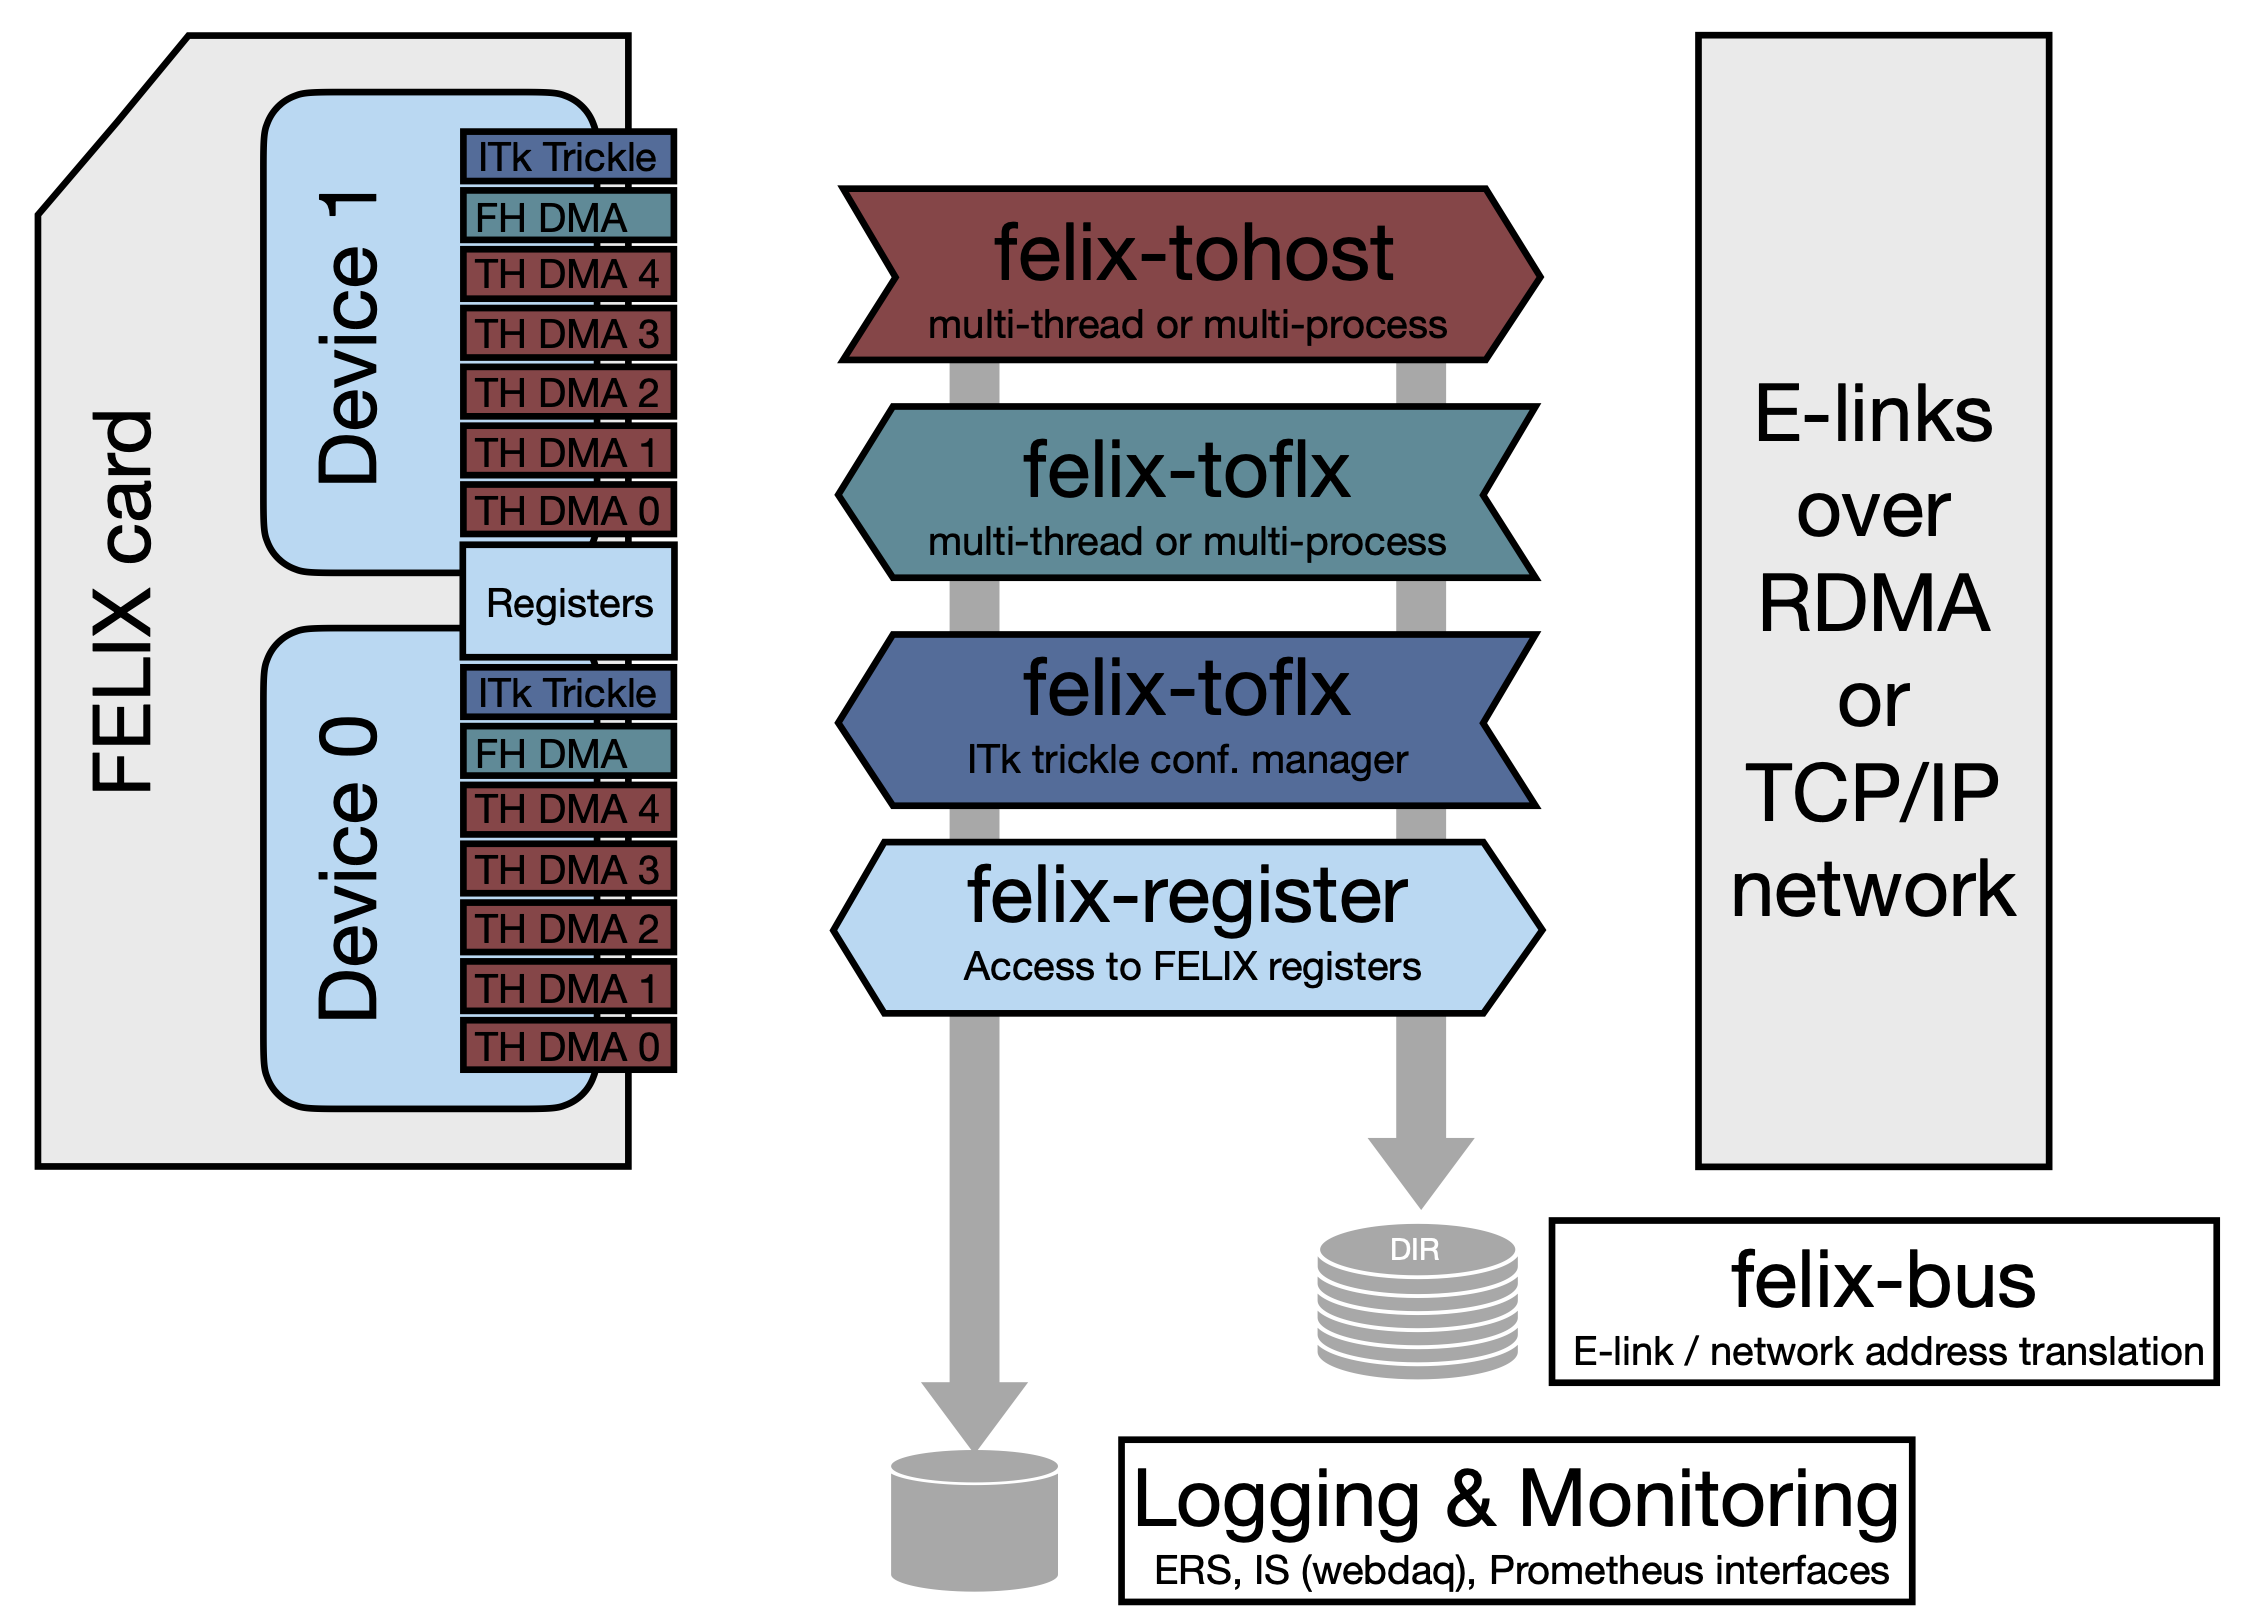
\includegraphics[width=0.8\textwidth]{images/felix/felix-star-architecture.png}
\caption{felix-star software architecture. The colours help understand what interacts with what. Briefly: felix-tohost reads from the same-coloured DMA buffers and sends the data over the network. felix-toflx does the opposite, takes data from the network and writes it into the DMA buffers. felix-register is used for RW operations on firmware registers. Image source \cite{felix-user-manual}}
\label{fig:felix-star}
\end{figure}

\clearpage
\section{FELIX-identifier}
\label{sec:felix_identifier}

\acs{E-link}s are identified by a 64-bit number called \ac{FID} \cite{fid}. Below is a definition of each field of the \acs{FID} followed by a visual representation.

\textbf{Version Identifier (VersionID):} The upper 4 bits of the FelixID, used to track revisions of the identifier format. Supports up to 16 versions, with 0x0 reserved for backward compatibility and 0x1 as the current version.

\textbf{Detector Identifier (DetectorID):} An 8-bit field that identifies the detector system. Allows for up to 255 detectors, aligning with the ATLAS Event Format.

\textbf{Connector Identifier (ConnectorID):} A 16-bit field that identifies fibre trunks (physical input units). Supports up to 65,536 connectors per detector, providing flexibility for future expansions.

\textbf{Link Identifier (LinkID):} A 14-bit field that distinguishes optical links within a fibre trunk. The highest bit is reserved for virtual links, leaving 13 bits for physical links, supporting up to 16,384 identifiers.

\textbf{Transport Identifier (TransportID):} A 14-bit field that subdivides links into logical E-links (for GBT mode) or indicates protocol and direction. Includes 6 bits for GBT E-Link ID, 1 bit for direction, and 7 bits for protocol, supporting up to 127 protocols.

\textbf{Stream Identifier (StreamID):} An 8-bit field that denotes specific streams within a link. Supports up to 255 streams per E-link or FULL mode link.


\begin{definition}
\label{def:FID}
\acs{FELIX}-identifier:

\begin{lstlisting}[caption={FELIX Identifier Fields}, label={lst:felix_identifier}]
+------------+--------------+------------+--------------+----------+---------+
|   4 bits   |    8 bits    |   16 bits  |    14 bits   |  14 bits |  8 bits |
+------------+--------------+------------+--------------+----------+---------+
| Version ID | Detector ID  | Connector  | Link ID      | Transport| Stream  |
|            |              | ID         |              | ID       | ID      |
+------------+--------------+------------+--------------+----------+---------+
\end{lstlisting}

\end{definition}

\section{felix-bus}
\label{sec:felix_bus}

\texttt{felix-bus} is a hierarchical structure of JSON files that provides the mapping between active E-links and network addresses. This mapping is essentially a way to translate a Detector-specific address into a more common network address. The directory containing felix-bus files must be accessible by all peers, this means that it should reside on a common network drive if communication occurs between different hosts.

A purpose of \texttt{felix-bus} is to minimize manual configuration of the \acs{FELIX} applications.
For example, client applications read from the felix-bus settings, like the number of network buffers and their size, and configure themselves accordingly.

The primary interface to felix-bus is the \texttt{felix-client-thread} \acs{API}. All references to “clients” in this context refer to applications using this \acs{API}.

\section{felix-tohost}

The application is responsible for reading data from \acs{DMA} transfer buffers --- that live inside the contiguous memory allocated by \texttt{cmem\_rcc} --- and send this data to the clients according to a publish/subscribe pattern. Multiple such applications may run on a single host. Each \acs{DMA} buffer is a circular buffer, with firmware and software monitoring and updating write and read pointers, respectively, to ensure that data is not overwritten.\\
The default behaviour is to spawn a single reader thread per \acs{DMA} buffer, but it is possible to configure the application to use multiple threads that can read each \acs{DMA} buffer.\\
\texttt{felix-tohost} supports both the physical hardware (felix-thost) and a simulation of it (felix-tohost2file).

\subsection{felix-tohost data format}

Event fragments or other types of data arriving via the FrontEnd links or virtual E-Links are referred to as “\texttt{chunks}” and can have an arbitrary size. Data inside the \acs{DMA} buffers is encoded in 1024-byte blocks. If a chunk is bigger than a block, it is divided in what is called a \texttt{subchunk}. Otherwise if a chunk does not completely fill a block, it is padded with zeroes and the whole block is sent after a timeout.\\
But why encode data in \texttt{blocks} and not directly use \texttt{chuncks}? Because having blocks makes the data easier for the software to handle: having a data format with a fixed size makes the memory alignment easier (constraint introduced by \acs{PCIe}), and similarly a fixed size makes \acs{DMA} much easier. Also there is an advantage for error handling discussed below in Subsection~\ref{sec:felix_tohost_error_handling}.

The typical processing sequence for felix-tohost is as follows:
\begin{itemize}
    \item The central event loop waits for a \texttt{data-available} signal (from \acs{FELIX} or via polling).
    \item A block is read from the contiguous memory buffer.
    \item The block header is checked for integrity, link identifier, and sequence number; out-of-order or invalid blocks are dropped and reported.
    \item Blocks are decoded into variable-length \emph{chunks}, handling incomplete chunks by combining sub-chunks across blocks as needed.
    \item Statistics are collected and monitoring data is published (Section~\ref{sec:felix_monitoring}).
    \item Completed chunks are sent to clients using the network library, either immediately (unbuffered) or after buffering (buffered mode).
    \item The buffer read pointer advances after chunk transfer or buffering.
    \item Processing pauses if the network is busy or the buffer is empty, resuming on new data or completion of network operations.
\end{itemize}

\subsection{Error Handling}
\label{sec:felix_tohost_error_handling}

Depending on the results of integrity checks, \texttt{flx-tohost} will drop entire blocks in certain cases to maintain overall system reliability and prevent corrupted data from causing problems in onward processing.\\
Currently in production can happen to receive corrupted data or data that is generated due to noise affecting Detector's electronics.
This is possible thanks to the existance of \texttt{blocks}. If --- inside a block --- a \texttt{chunk}'s header is corrupted the payload size shown is often very big, but blocks have a fixed size of 1KB, so at most 1KB of data is lost and there is no need for more sophisticated error detection and correction mechanisms.

\section{felix-toflx}
\label{sec:felix_toflx}
\texttt{felix-toflx} provides the complementary data path to \texttt{felix-tohost}. \texttt{felix-tohost} receives data from the network destined to the \acs{E-link}s that have been enabled, writes them in the designated \acs{DMA} buffers, and ultimately the \acs{FELIX} card transfers the data to those \acs{E-link}s which will correspond to \acl{FE} electronics.
Similar to \texttt{felix-tohost}, this component supports both physical hardware (felix-toflx) and a simulation of it (felix-toflx2file).\\
Unlike \texttt{felix-tohost} which uses publish/subscribe patterns, felix-toflx employs a send/receive pattern for network communication.

\subsection{felix-toflx data format}

The data format is different compared to \texttt{felix-tohost}. First the blocks can be 256, 512, or 1024 bits, depending on the \acs{PCIe} generation (gen 3, 4 and 5). Each block always contains a header of 32 bit and this header only contains the \acs{E-link} ID of a \acl{FE} destination and the size of the payload.

\section{Trickle Configuration}

The on-detector electronics of \acf{ITk} are radiation-tolerant, but nevertheless they tend to lose their configuration with time due to \acl{SEU} induced by high levels of radiations \cite{buschmann2019itk} of the environment in which they operate.\\
\texttt{Trickle Configuration} is the \texttt{felix-star} application that sends the configuration towards the \acl{FE} electronics, which means that all configurations (global and pixel) can be gradually updated during operation by continually sending write commands in between triggers. This avoids the need to also have configuration registers to be \acs{SEU}-hard.\\
The direction of the data for \texttt{Trickle Configuration} is the same as of \texttt{felix-toflx}.

\section{Logging and Monitoring}
\label{sec:felix_monitoring}

As seen in the previous sections, \texttt{felix-star} applications are responsible for monitoring and logging their activities. The monitoring system is designed to be flexible and extensible, allowing for different output formats and destinations.\\
The monitoring system is based on JSON formatted messages.\\
Monitoring information produced by \texttt{felix-star} applications can be exported in 3 different ways:

\paragraph{Grafana} \texttt{felix-star} can output the data directly into Prometheus \cite{prometheus} from which Grafana \cite{grafana} queries the information that will be displayed.

\paragraph{FIFO} \texttt{felix-star} can output the data into a UNIX FIFO.

\paragraph{\ac{IS}} \texttt{felix-star} can output the data into \acs{IS} \cite{is}, a monitoring system used internally in \acs{ATLAS}.\\

The logging system of \texttt{felix-star} applications is \acf{ERS} \cite{ers}. \acs{ERS} software package provides a common \acs{API} for error reporting in the \acs{ATLAS} \acs{T-DAQ} system. \acs{ERS} offers several macros that can be used for reporting pre-defined errors if some conditions are violated; below a list of available macros:

\begin{itemize}
    \item \texttt{ERS\_ASSERT(expression)}: A generic macro that checks whether a given expression is valid.
    \item \texttt{ERS\_PRECONDITION(expression)}: The same as \texttt{ERS\_ASSERT} but uses a user-defined message to be reported.
    \item \texttt{ERS\_RANGE\_CHECK(min, val, max)}: A special type of pre-condition, which checks that a value is in a closed range between \texttt{min} and \texttt{max} values.
    \item \texttt{ERS\_STRICT\_RANGE\_CHECK(min, val, max)}: Similar to \texttt{ERS\_RANGE\_CHECK} but does not allow the checked value to be equal to either \texttt{min} or \texttt{max} values.
\end{itemize}

\acs{ERS} also provides tools for defining custom classes that can be used for reporting user-defined issues. 

\begin{lstlisting}[language=C++, caption={ERS Assertion Issue Declaration}, label={lst:ers_assertion_issue}]
ERS_DECLARE_ISSUE(
    ers,                                                          // namespace
    Assertion,                                                    // issue name
    "Assertion (" << condition << ") failed because " << reason,  // message
    ((const char *)condition )                                    // first attribute
    ((const char *)reason )                                       // second attribute
)
\end{lstlisting}

The \acs{ERS} \acs{API} offers multiple functions, each corresponding to a specific severity level, for reporting custom issues. Issues logged to \acs{ERS} streams can be forwarded to different destinations based on the stream configuration. By default, \acs{ERS} streams are configured as follows:

\begin{itemize}
    \item \texttt{ers::debug()} - \texttt{"lstdout"}: Prints issues to the standard C++ output stream.
    \item \texttt{ers::log()} - \texttt{"lstdout"}: Prints issues to the standard C++ output stream.
    \item \texttt{ers::info()} - \texttt{"throttle,lstdout"}: Prints throttled issues to the standard C++ output stream.
    \item \texttt{ers::warning()} - \texttt{"throttle,lstderr"}: Prints throttled issues to the standard C++ error stream.
    \item \texttt{ers::error()} - \texttt{"throttle,lstderr"}: Prints throttled issues to the standard C++ error stream.
    \item \texttt{ers::fatal()} - \texttt{"lstderr"}: Prints issues to the standard C++ error stream.
\end{itemize}

\acs{ERS} is thread-safe and is used for error reporting in multi-threaded applications.\\
Lastly, \acs{ERS} provides an interface to export and store the loggings.

\clearpage
\section{Personal Contributions}


\subsection{Trickle Configuration - Software Architecture}

\texttt{Trickle configuration} \cite{felix-star-trickle-configuration} has been implemented as a layer on top of the existing (but enhanced for the purpose) buffer and device handler in the \texttt{felix-toflx} direction. In the image~\ref{fig:trickle-software-architecture} below there is a simple representation of the software architecture, while a complete UML diagram is in Figure~\ref{fig:complete-monitoring-uml} in the Appendix A~\ref{ch:appendix}. As per usual there is the possibility to run trickle on the real hardware or as an emulator; the emulators in the \texttt{felix-star} suite are mainly used for regression testing, for debugging the actual hardware is preferred, but that is not a rule.

\begin{figure}[htbp]
\centering
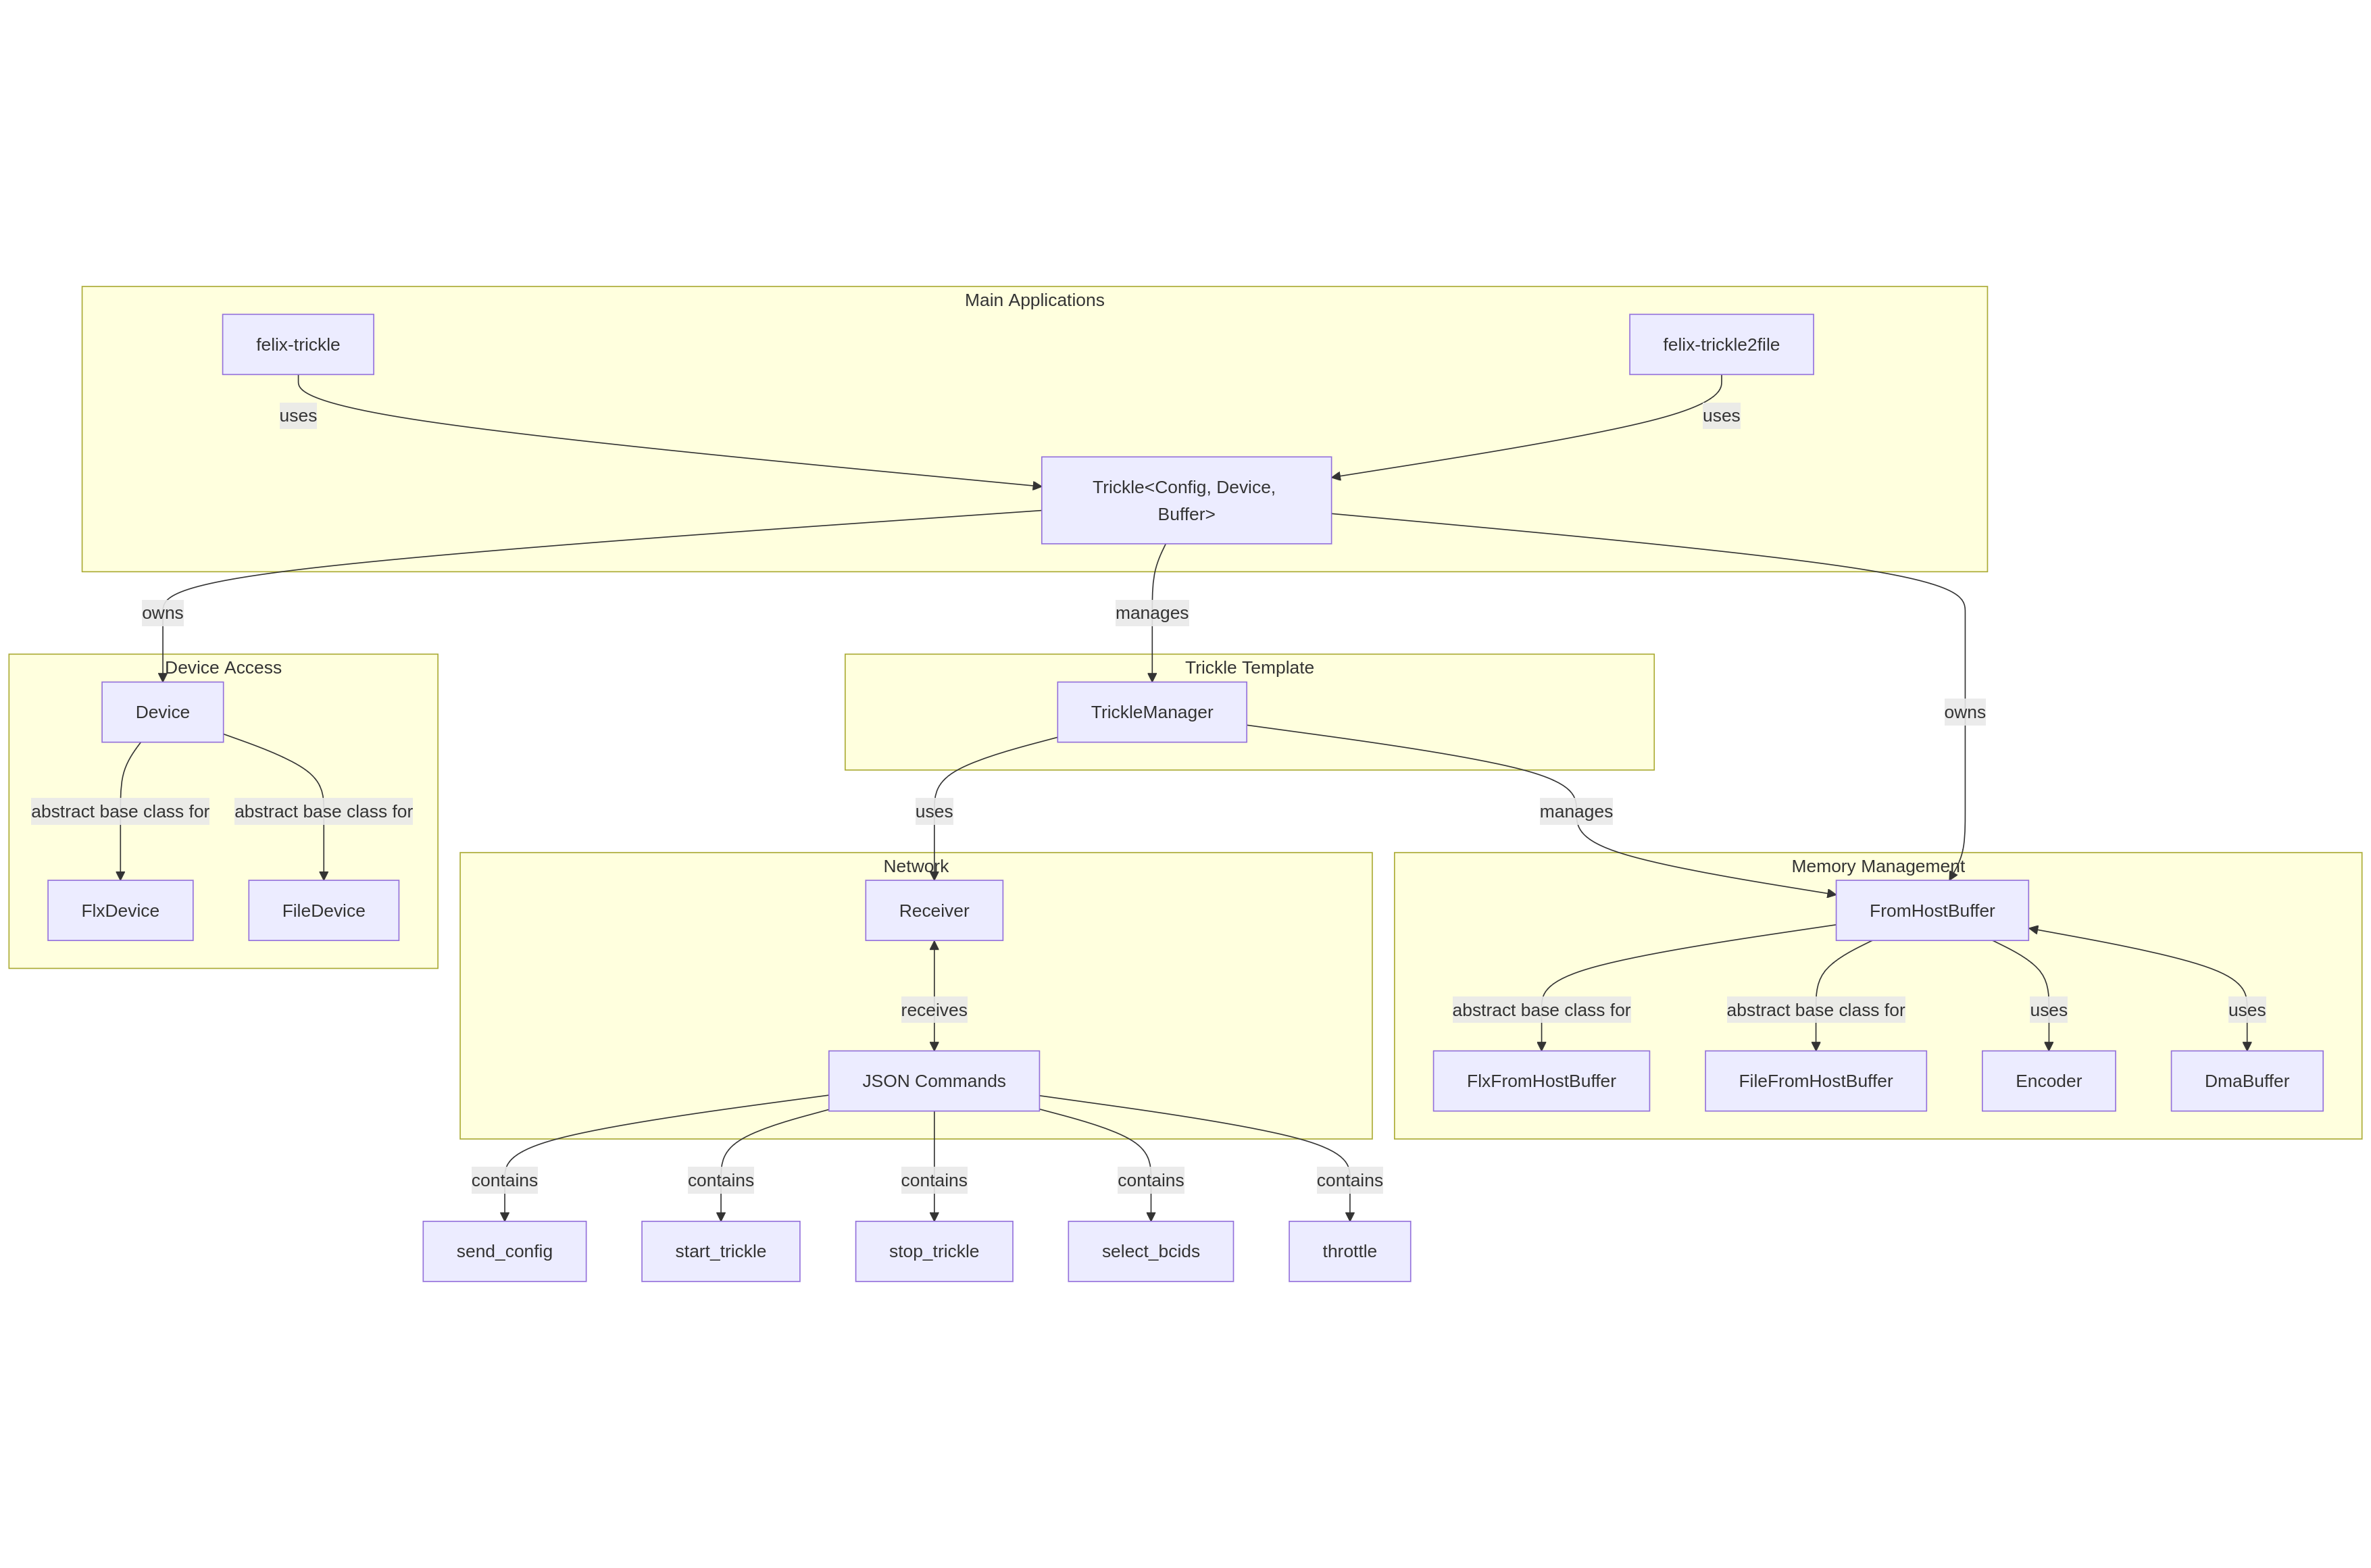
\includegraphics[width=\textwidth]{images/contributions/trickle-architecture.png}
\caption{Software architecture of Trickle configuration.}
\label{fig:trickle-software-architecture}
\end{figure}

\subsection{Software Flow Example}
\begin{enumerate}
    \item Configuration data is received with \textit{send\_config}.
    \item \textit{start\_trickle} starts the "trickling" process.
    \item Host software encodes and writes the payload into the Trickle ring-buffer. The host may add padding for memory alignment (e.g., 4096-byte alignment), a requirement derived from the \acs{PCIe} standard.
    \item Firmware periodically reads from the buffer, sending configuration to the \acs{FE} electronics in between triggers.
    \item \textit{stop\_trickle} stops the "trickling" process.
\end{enumerate}

\subsubsection{felix-trickle} is the name of the main executable (the source file is main\_trickle.cpp) that runs \texttt{trickle\ configuration} on a \acs{FELIX} card. It is responsible for instantiating a \emph{Trickle} instance with the configuration parameters, all the \acs{FELIX} devices installed on the host, and the \acs{DMA} buffers that will be written by the software and read by the firmware. It is responsible for starting or stopping the trickling process through the \emph{Trickle} instance, and for capturing and handling any kernel signals.

\subsubsection{felix-trickle2file} is the name of the main executable (the source file is main\_trickle2file.cpp) that runs \texttt{trickle configuration} in a simulated environment. It is used for regression testing and debugging purposes. It is responsible for instantiating a \emph{Trickle} instance with the configuration parameters, all the emulated \acs{FELIX} devices, and the \acs{DMA} buffers that in this case will be read by an emulator of the firmware and, if the user configured it, written to a file. It is responsible for starting or stopping the emulated trickling process through the \emph{Trickle} instance, and for capturing and handling any kernel signals.

\subsubsection{Trickle} is the class that depending on the configuration parameters and the type of \acs{FELIX}, will be able to perform the trickling operation with the real hardware or an emulated one. It owns, by composition, \acs{FELIX} devices and \acs{DMA} buffers.\\
It is responsible for setting the correct data format with witch to fill the \acs{DMA} buffers, to actually allocate the memory for the \acs{DMA} buffers, to publish the data into the \emph{felix-bus} so that the \emph{felix-clients} can communicate with the application, and finally to instantiate a \emph{TrickleManager} instance for each \acs{FELIX} device and an unbuffered \emph{Receiver} per buffer.

\subsubsection{TrickleManager} is the class that implements the \acs{API} that allows to use \texttt{trickle configuration}. The \acs{API} is composed of the following functions:
\begin{itemize}
    \item \texttt{send\_config}: Sends the configuration data to the \acs{FELIX} card.
    \item \texttt{start\_trickle}: Starts the trickling process.
    \item \texttt{stop\_trickle}: Stops the trickling process.
    \item \texttt{select\_bcids}: Selects the bunch crossing IDs in which to send the config messages.
    \item \texttt{throttle}: Throttles the trickling process.
\end{itemize}

It uses a \texttt{Receiver}~\ref{subsubsec:receiver} to receive commands in JSON format from a client, and each command uses one of the aforementioned functions.\\

\texttt{select\_bcids} merits some explanation. In the \acl{LHC} there are two directions in which particles can circle; the particles are divided in "bunches" inside a beam, the collisions happen always between the same bunches in the crossing points that correspond to the four experiments presented in the introduction~\ref{sec:lhc-experiments}, and this collision will have an ID which is the \acl{BCID}. \emph{Trickle configuration} is supposed to send data in between triggers, which happen when the bunches cross, so with \emph{select\_bcids} one can theoretically select only the IDs preceding longer periods without collisions. The effect of selecting \acs{BCID}s is that of throttling, for which there is a function implemented in the \acs{API}, but both of them have been kept since they are two different concepts even though they have the same final effect.\\
A reference to a tool to simulate bunch crosses inside the \acs{LHC} \cite{bunch-crossing-tool}.

There are private implementations of the callback functions that are used to handle the events of opning/closing a connection and receiving data. There is also a function that adds padding to a \emph{trickle configuration} payload to ensure that the data is aligned to a 4096-byte boundary, which is a requirement of the latest \acs{PCIe} standard. The interesting part is that the padding needs to actually be a valid message for the firmware to be able to read it. The final implementation consists on adding a header that contains a valid \acs{E-link} but an invalid E-path. Since then the firmware has been developed to simply ignore and discard messages with headers containing invalid \acs{E-link}s.

\subsubsection{FromHostBuffer} is the abstract base class that is tasked with managing buffers in the \texttt{felix-toflx} direction. It is specialized to work both with the real hardware and with the emulated one. It is responsible keeping track of the read and write pointers to the \acs{DMA} buffer it is wrapping, and to manage concurrent \emph{write} and \emph{read} operations to it.

\subsubsection{Device} is the abstract base class that represents a \acs{FELIX} device. It is responsible for managing the connection to the \acs{FELIX} card, and for providing an interface to read and write registers. It is specialized to work both with the real hardware (1 object = 1 \acs{PCIe} endpoint) or to emulate one. The class is used by \emph{TrickleManager} to access the \acs{FELIX} card or the emulated one.\\

\subsubsection{Receiver} \label{subsubsec:receiver} is the interface implemented by the network backed that the trickle software uses to receive data from the network.

\subsection{Firmware's role}

The \acs{FELIX} firmware is responsible for reading configuration data from the Trickle buffer and forwarding it to the appropriate \acs{FE} links. The read pointer in firmware advances as configuration data is consumed. No write pointer is maintained in firmware; the reason behind the pointers choice is because \textit{trickle configuration} is something that will not change often, it is meant to be written one time in the \acs{DMA} buffer with the firmware continuously reading the buffer and sending the configuration in between triggers. When the configuration needs to change, the buffer is set to one-shot (which invalidates the buffer once reading the last bit), the confiuration is changed, the buffer is again set to be a ring-buffer and the firmware is given the signal to start reading again by setting the register that validates the buffer.\\
The firmware is implemented in a way so that \texttt{trickle configuration} has the lowest priority compared to other data.

\subsection{Trickle Configuration - Client}

Image~\ref{fig:trickle-client-uml} how the \texttt{Trickle Configuration} \acs{API} call has been implemented on the client side \cite{felix-star-trickle-client}. 

\begin{figure}[htbp]
\centering
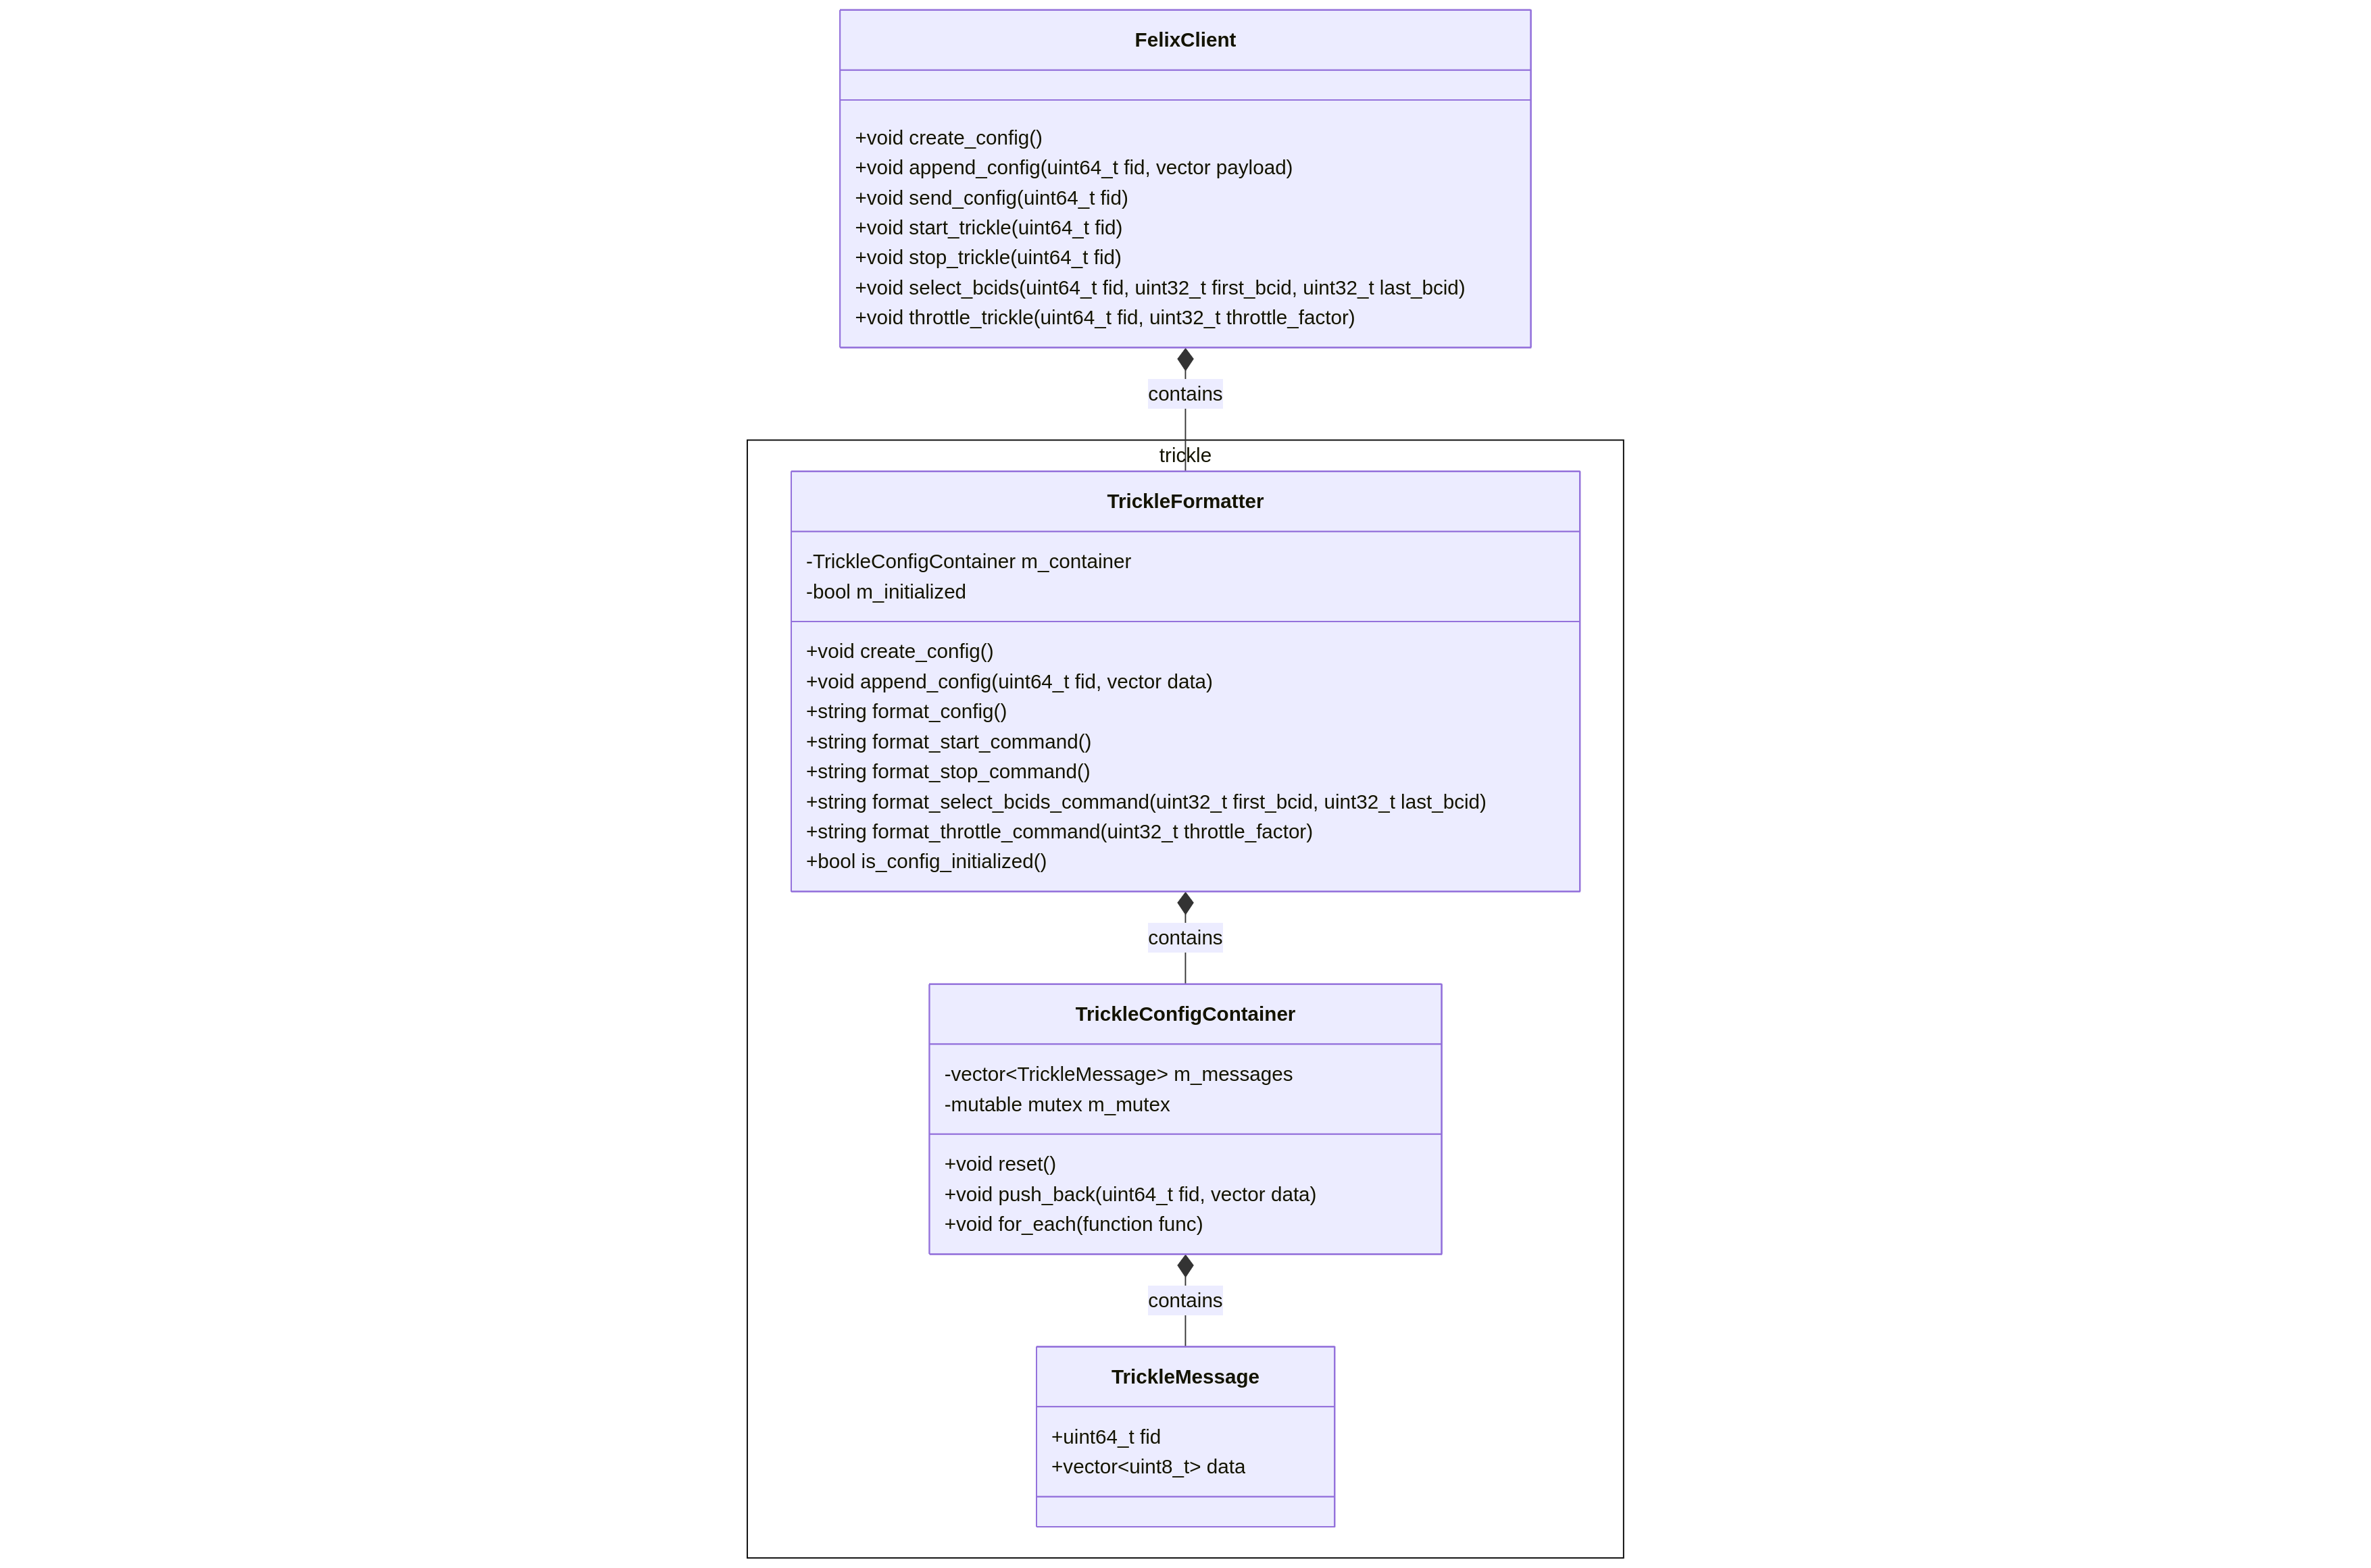
\includegraphics[width=\textwidth]{images/contributions/client-trickle-config-uml.png}
\caption{UML diagram Trickle Configuration in the client side.}
\label{fig:trickle-client-uml}
\end{figure}

A brief explanation of the classes involved in the client-side implementation of the \texttt{Trickle Configuration} \acs{API}:

\begin{itemize}
    \item \textbf{TrickleMessage}: An internal structure that represents a single Trickle configuration message. It contains the \acs{FID} and the payload.
    
    \item \textbf{TrickleConfigContainer}: A container for \texttt{TrickleMessage} structs. Its role is to provide a thread-safe storage and manipulation of trickle messages.
    
    \item \textbf{TrickleFormatter}: This class is responsible for formatting trickle messages into JSON strings.
    
    \item \textbf{FelixClient}: This is the class that implements the \acs{API} to interact with the \texttt{felix-star} applications. It is responsible for sending and receiving messages, and for managing the connection to the \texttt{felix-star} applications. In the context of \texttt{trickle configuration} it uses the \texttt{TrickleFormatter} generate trickle configurations in JSON format, and generate commands to send to the server, also as JSON strings.
\end{itemize}

\clearpage
\subsection{Monitoring - Software Architecture}

Initially, the \acs{FELIX} monitoring system was structured around a \texttt{Monitor} class, which provided a \texttt{write\_message()} method. This method was inherited and overridden by subclasses such as \texttt{FromHostMonitor} and \texttt{ToHostMonitor}. While this approach allowed for some specialization, it tightly coupled the monitoring logic with the output mechanism, making it difficult to introduce new output formats or destinations without modifying the core monitoring classes.

To address these limitations, the architecture was refactored to apply the \textit{Strategy design pattern}. Figure~\ref{fig:monitoring-software-architecture} shows a UML diagram of the most important parts composing the \textit{Monitoring} implementation; a complete UML diagram is in Figure~\ref{fig:complete-monitoring-uml}. The Strategy pattern allows selecting an algorithm's behavior at runtime by encapsulating it within a separate class and delegating the execution to that class.

\begin{figure}[htbp]
\centering
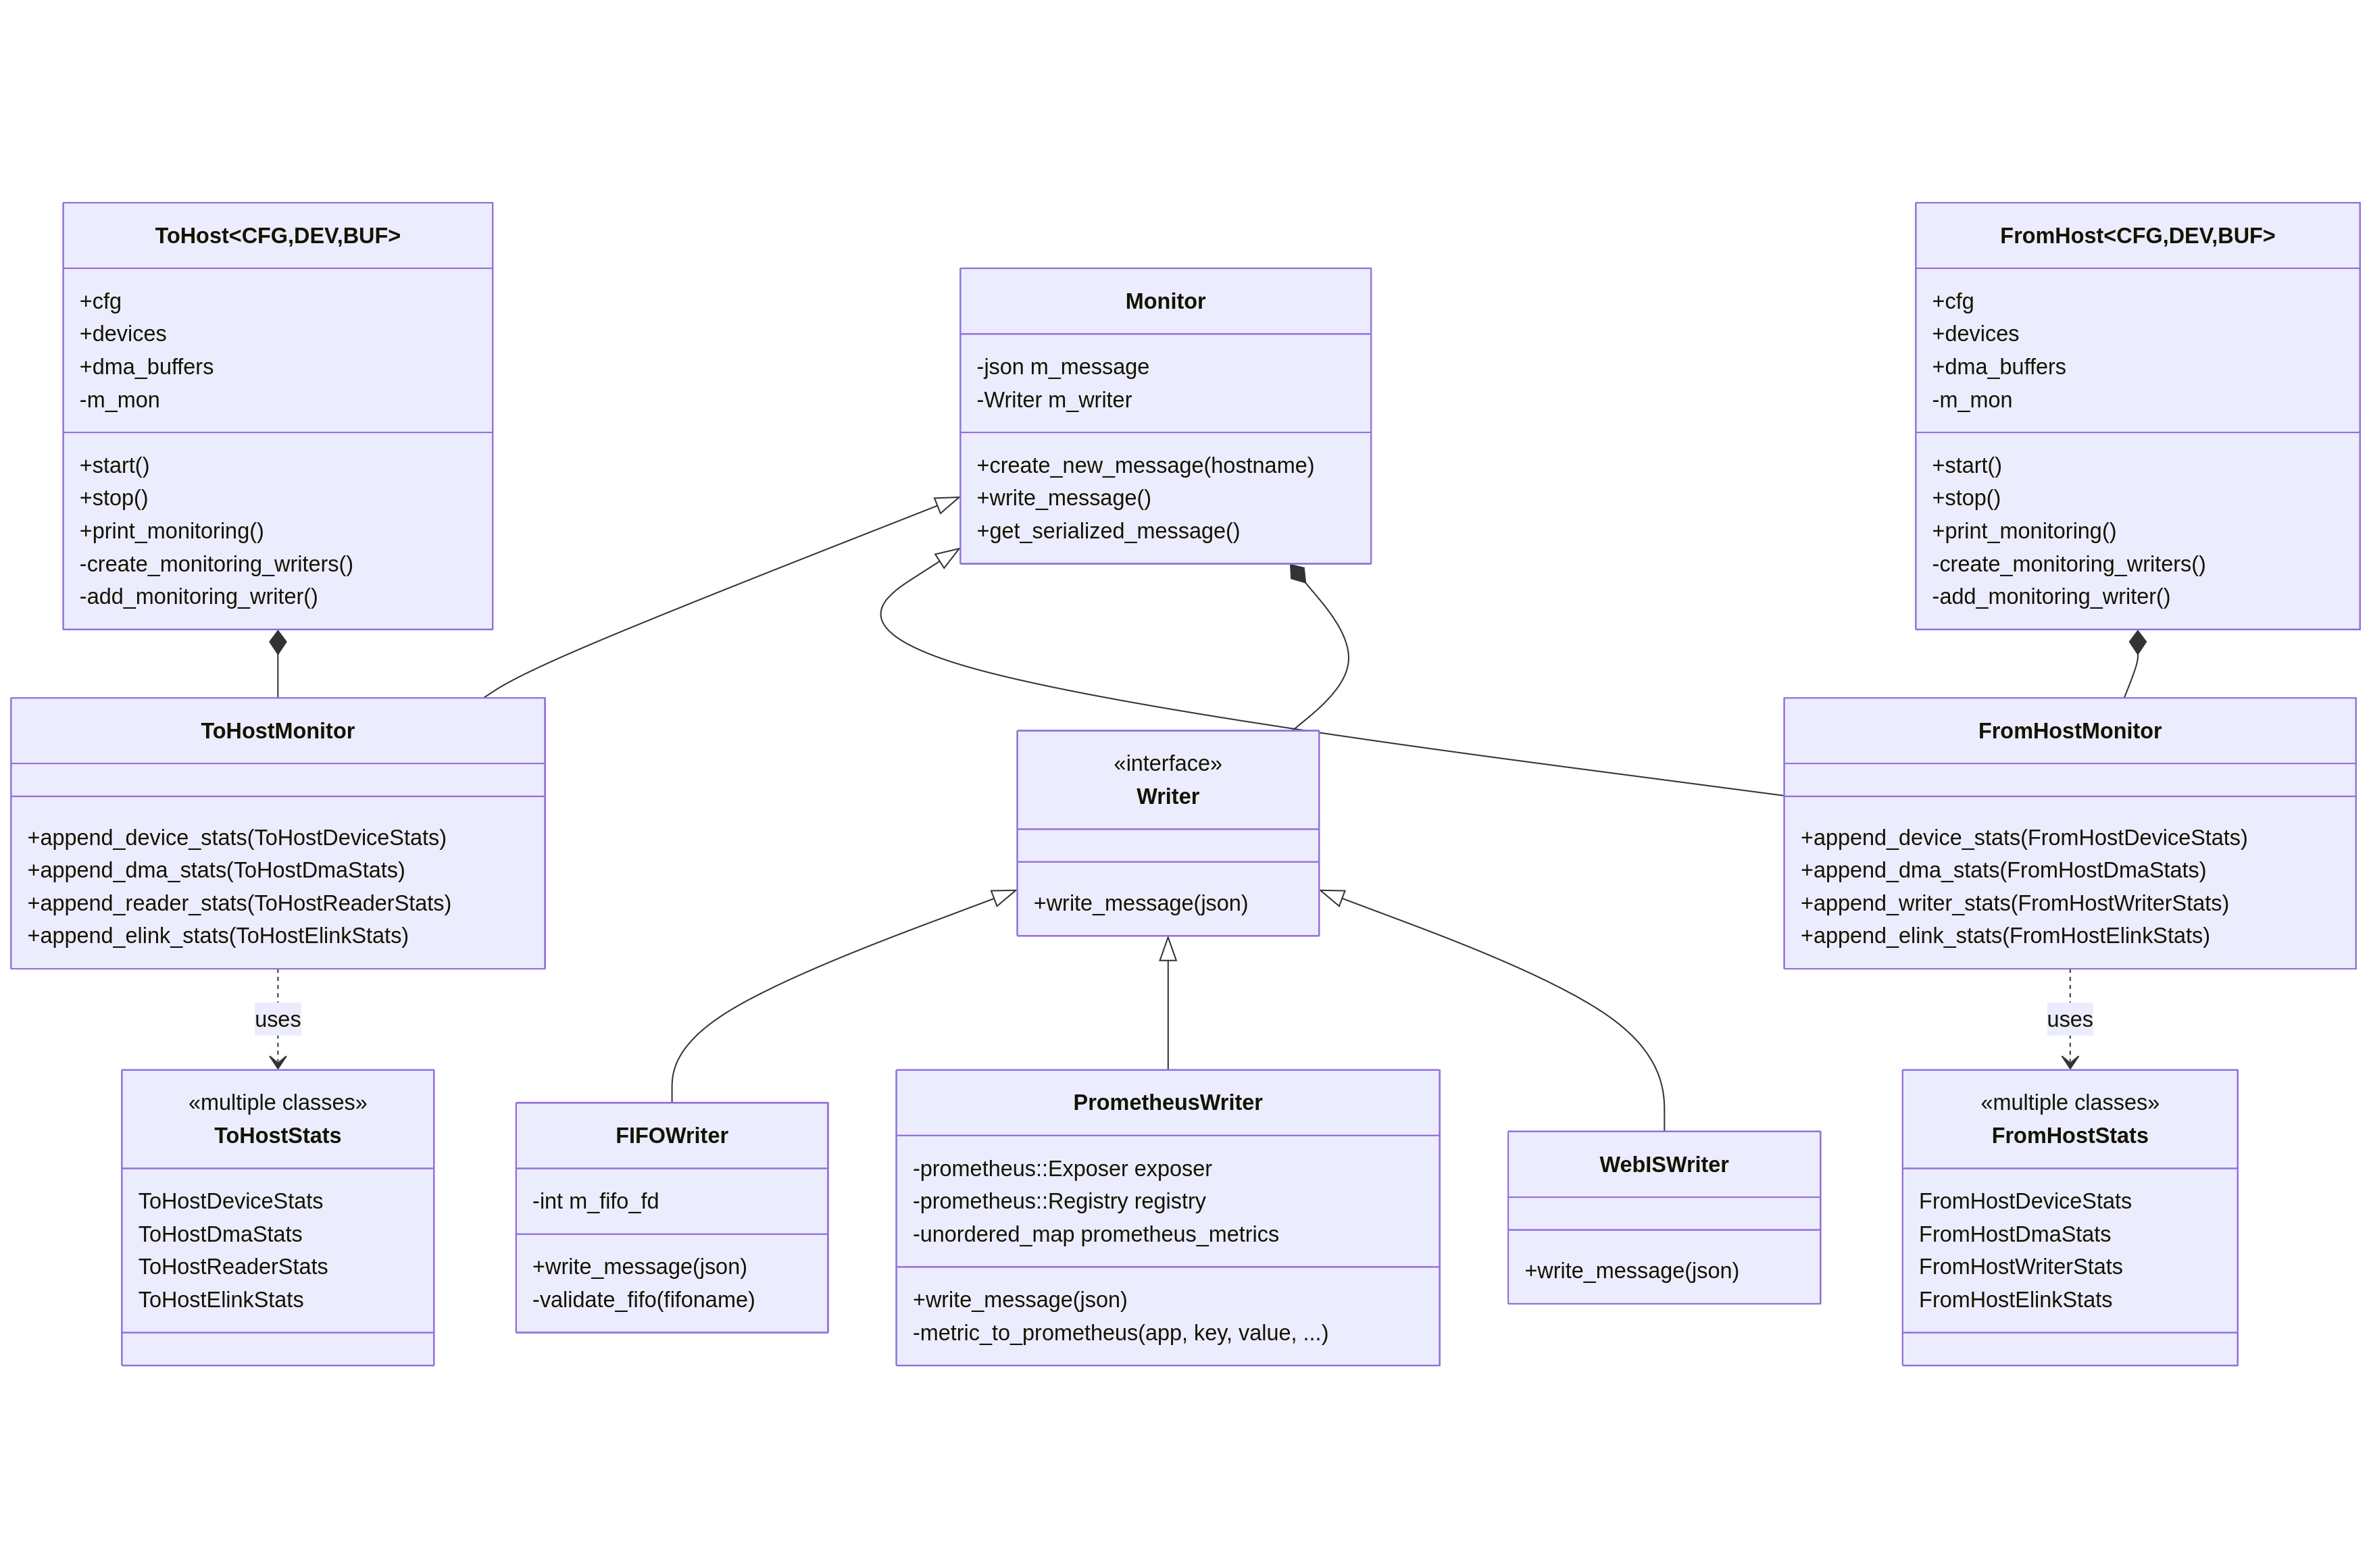
\includegraphics[width=\textwidth]{images/contributions/monitoring-uml.png}
\caption{Overview of the monitoring software architecture.}
\label{fig:monitoring-software-architecture}
\end{figure}

\textbf{Monitor} is the class that is used by the \texttt{felix-star} applications to produce monitoring data. It is an abstract base class that defines the interface for monitoring. It has a pure virtual method \texttt{write\_message(const nlohmann::json\&)} that must be implemented by subclasses. The \texttt{Monitor} class is responsible for collecting monitoring data and delegating the writing of that data to a \texttt{Writer} instance. The concrete implementations are defined depending on the direction, thus there are \emph{ToHostMonitor} and \emph{FromHostMonitor} .The choice of \texttt{Writer} implementation is determined at runtime based on user configuration, allowing the same monitoring logic to be reused with different output strategies.

\textbf{Writer} is the abstract base class for the three concrete implementations of the monitoring output strategies. Each of the concrete classes implements the \texttt{write\_message(const nlohmann::json\&)} method, which defines how the monitoring data is written to the desired output or destination. The concrete implementations of this class include:

\begin{itemize}
    \item \textbf{FIFOWriter}: Writes monitoring data to a UNIX FIFO (Figure~\ref{fig:fifo-monitoring}).
    \item \textbf{PrometheusWriter}: Exposes metrics in a format consumable by Prometheus (Figure~\ref{fig:felix-tohost-monitoring}, Figure~\ref{fig:felix-tohost-single-elink}).
    \item \textbf{WebISWriter}: Used to send monitoring data to \acs{IS}, a monitoring tool used internally in \acs{ATLAS} (Figure~\ref{fig:felix-tohost-is}).
\end{itemize}

\begin{figure}[H]
\centering
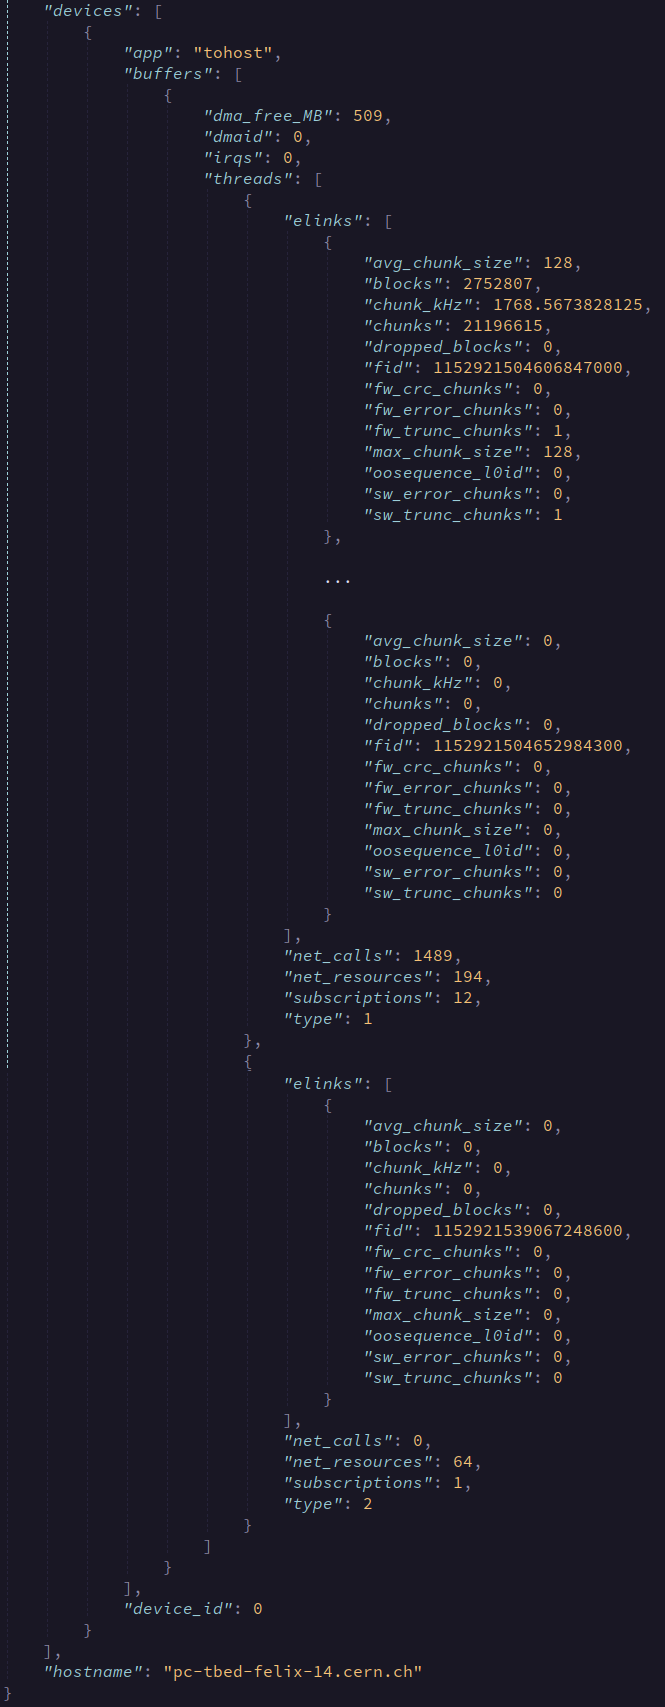
\includegraphics[width=0.46\textwidth]{images/results/fifo-monitor.png}
\caption{An example of what can be seen inside the UNIX FIFO. It's a JSON message containing the monitoring data.}
\label{fig:fifo-monitoring}
\end{figure}

\begin{figure}[H]
\centering
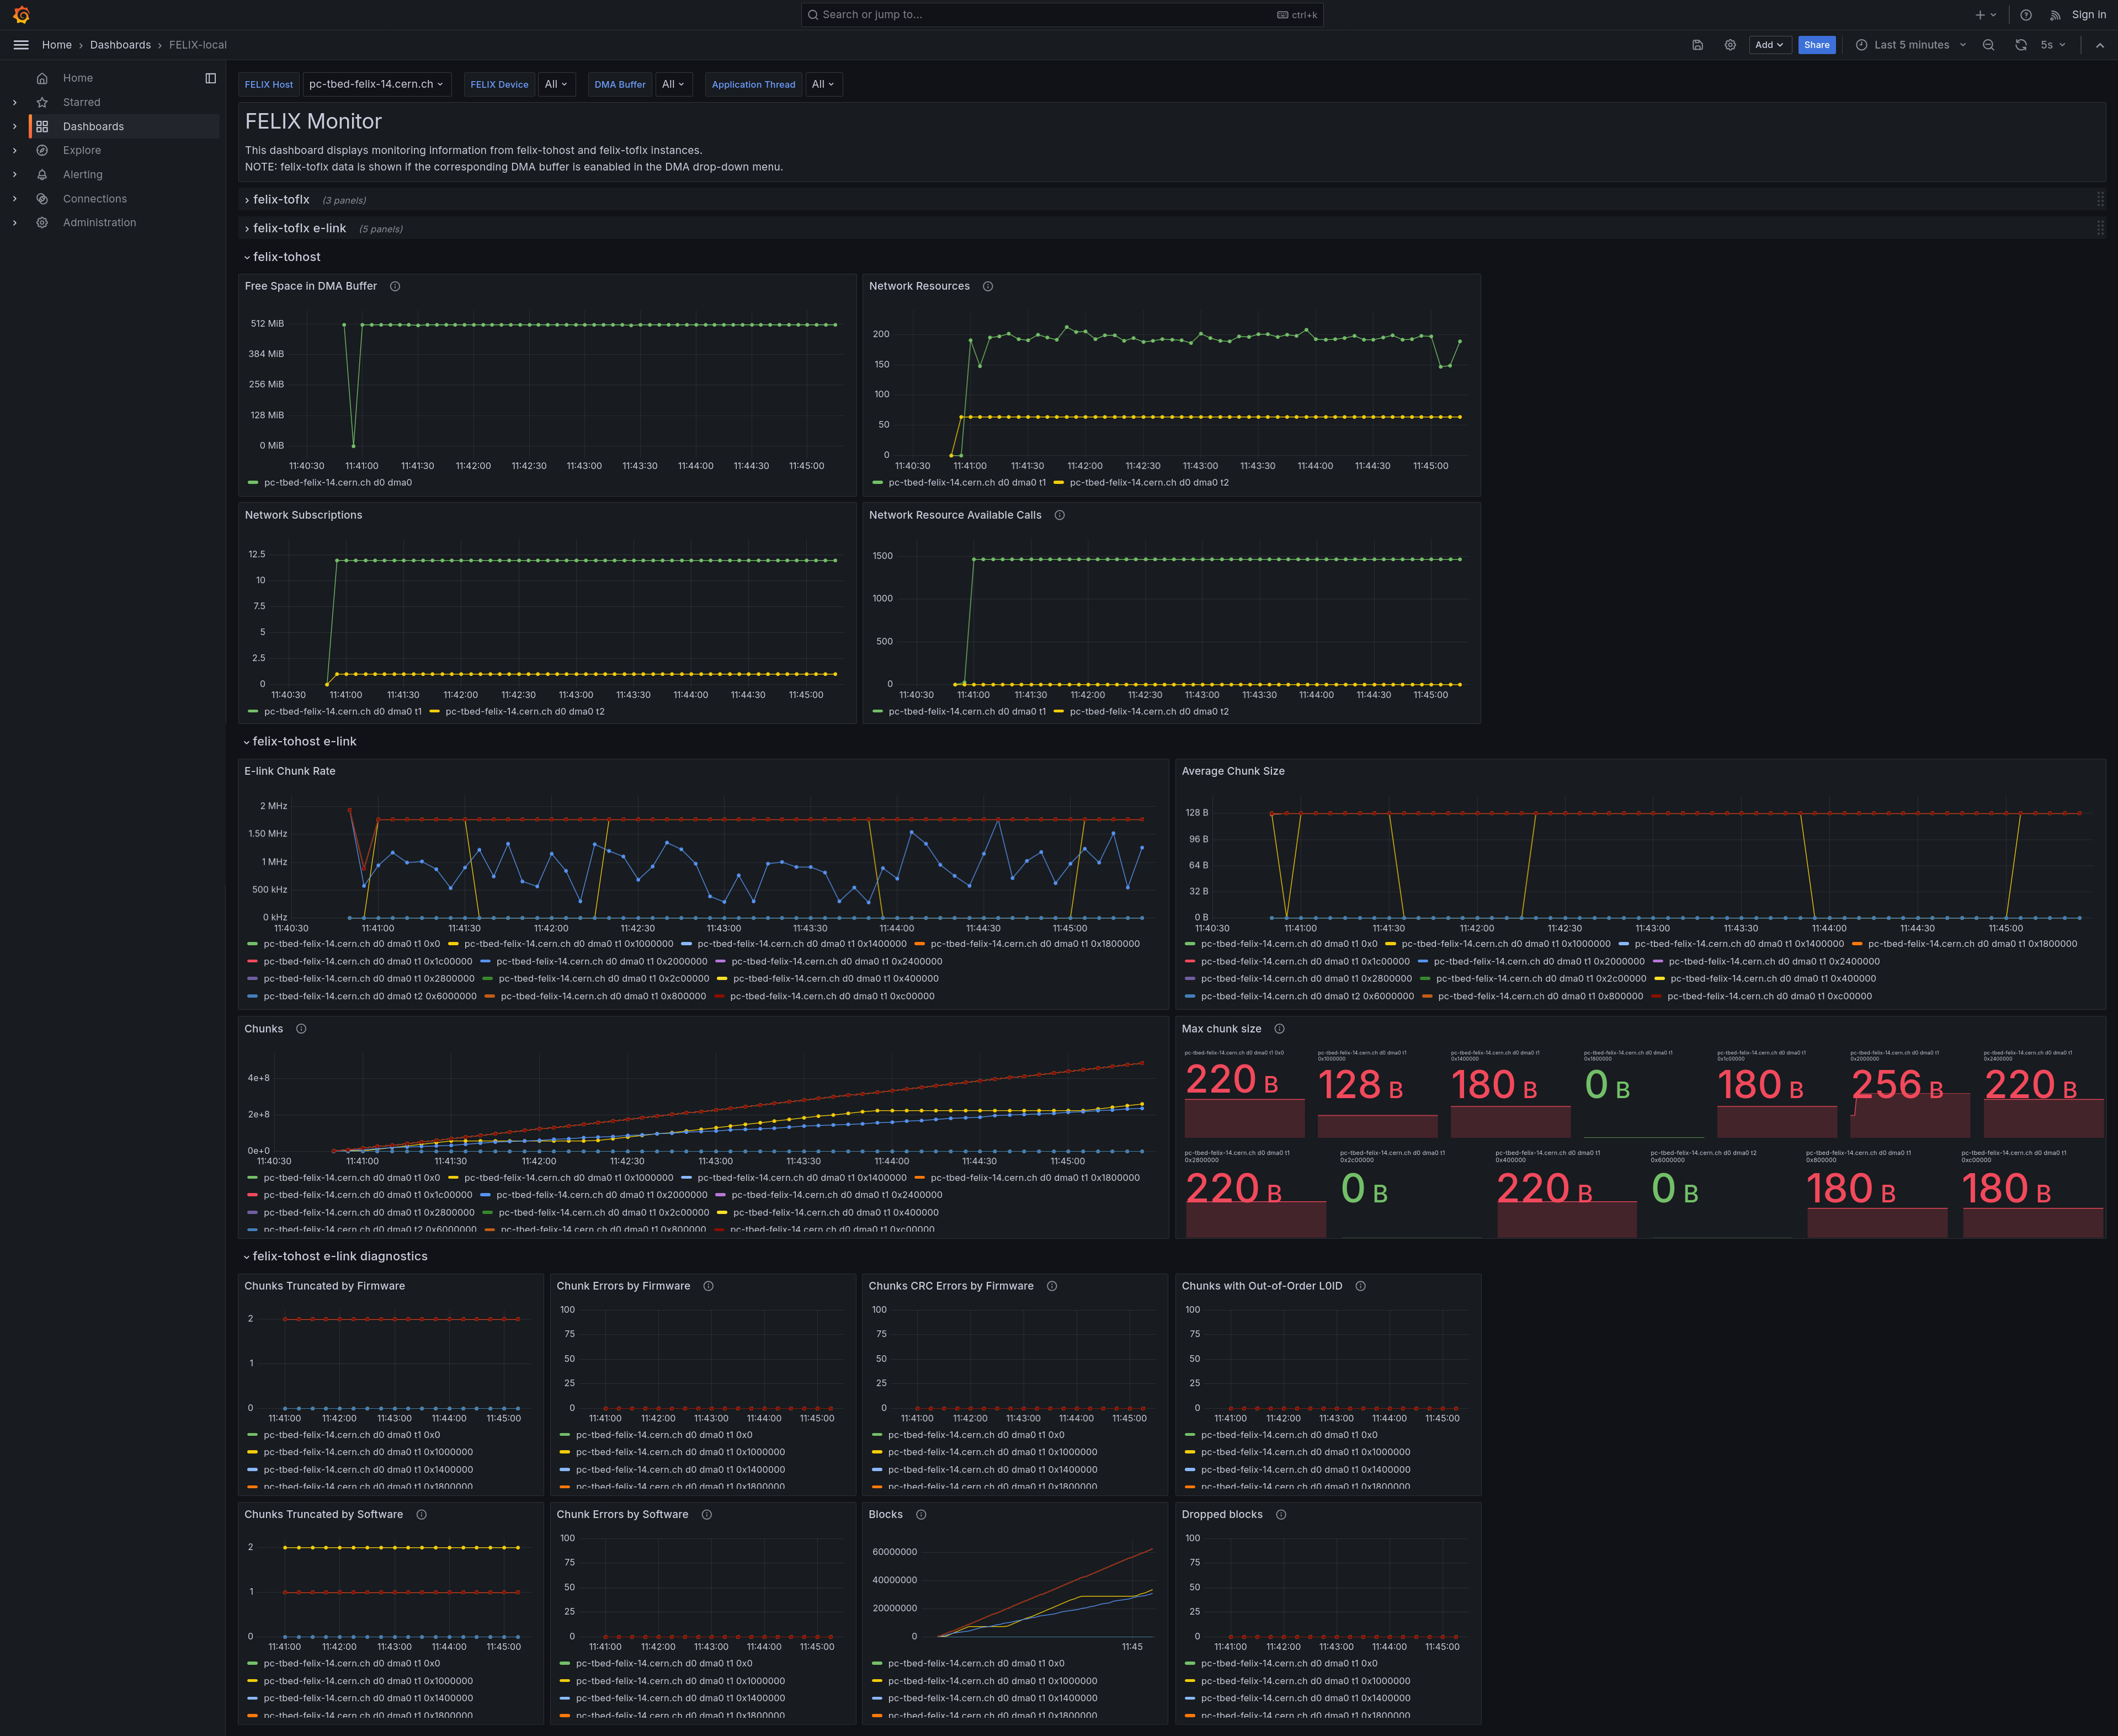
\includegraphics[width=\textwidth]{images/results/monitoring-merged.png}
\caption{This is a sample screenshot of the combined Prometheus and Grafana solution. The sampling rate can be set in the docker image, in this case it is 5 seconds. Here I was stress testing felix-tohost as shown by the size of the chunks and their \acs{E-link} rate well above 1.5 MHz. }
\label{fig:felix-tohost-monitoring}
\end{figure}

\begin{figure}[H]
\centering
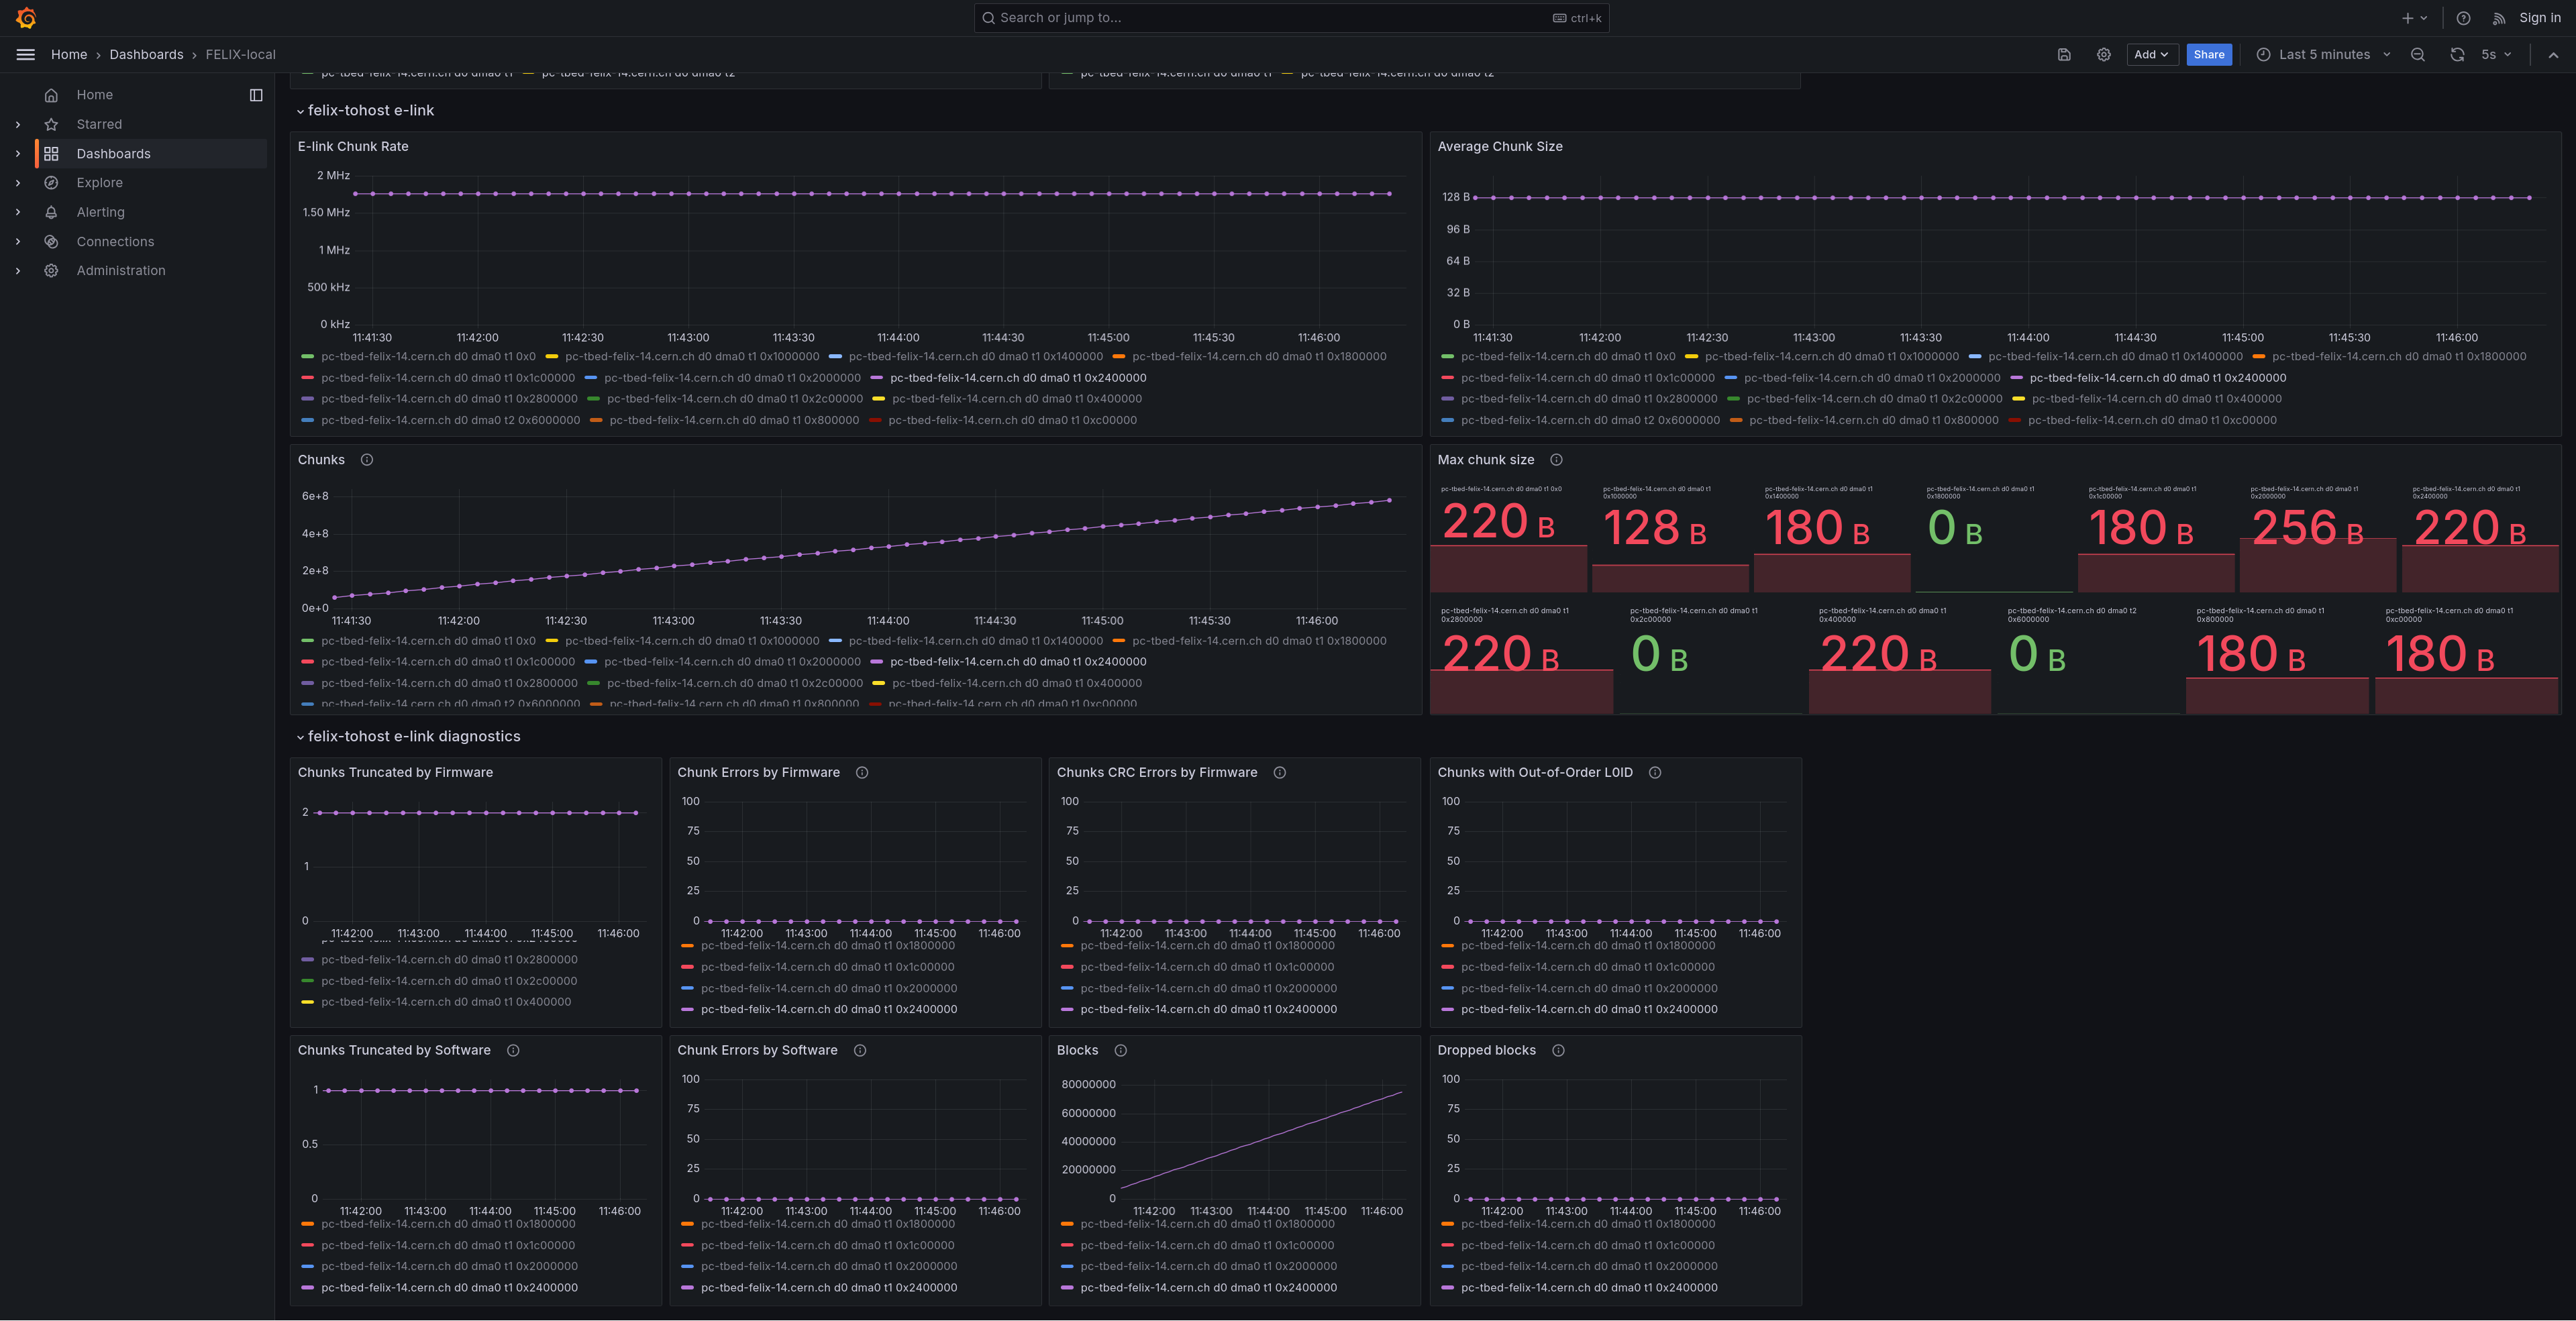
\includegraphics[width=\textwidth]{images/results/monitor-one-elink.png}
\caption{Here a screenshot showing that it is possible to select and focus one element at a time, in this case I selected the \acs{E-link} 0x2400000.}
\label{fig:felix-tohost-single-elink}
\end{figure}

\begin{figure}[H]
\centering
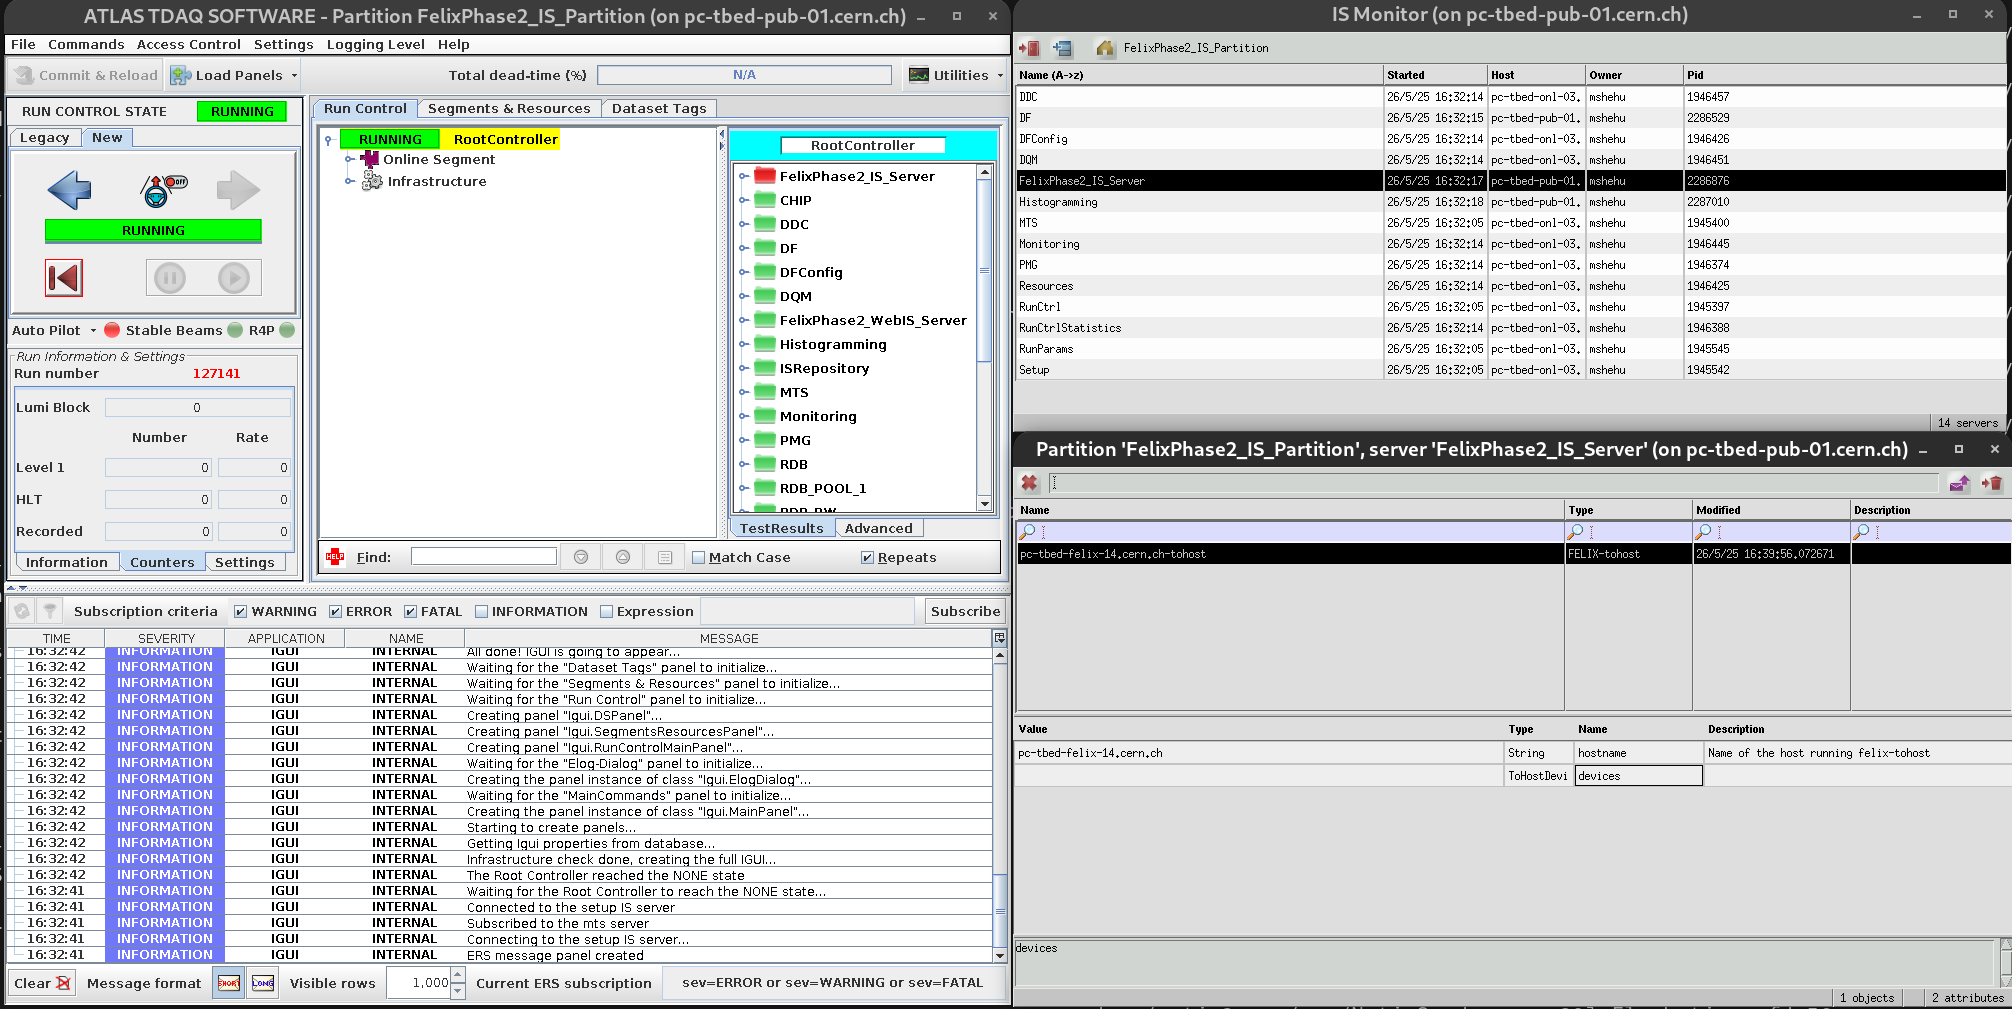
\includegraphics[width=\textwidth]{images/results/IS-monitoring.png}
\caption{Sample image with IS monitoring. The reason that it is red is because it's trying to test it but there is no test available since this is just a play setup to check if it works.}
\label{fig:felix-tohost-is}
\end{figure}


\subsection{Migration of the logging system from clog to ERS}

The contribution in this matter is straightforward: the logging system has been migrated from \texttt{clog} to \texttt{ERS}. The purpose of this migration is to make \texttt{felix-star} consistent and coherent with the \acs{ATLAS} \acs{T-DAQ} software ecosystem \cite{felix-star-clog-to-ers}.\\
Contrary to the approach of other software using ERS, for \texttt{felix-star} I decided to create a general issue per Class, and specialize the issue with a custom message depending on the situation.\\
Below an Example~\ref{lst:ers-example} of an actual implementation:

\begin{lstlisting}[language=C++, caption={Example of ERS custom issue declaration and usage.}, label={lst:ers-example}]
/* In the header file */
// Declare a custom issue for logging configuration-related errors
ERS_DECLARE_ISSUE(felix_log, device_flx_issue, issue_message, ((const std::string&)issue_message))

/* In the cpp file */
// Use the custom issue to log an error
ers::error(felix_log::device_flx_issue(std::format("Invalid encoding type {} for elink channel {} group {}, epath {} using DIRECT", enc, channel, egroup, epath)));
;
\end{lstlisting}